\documentclass%
%[handout]
{beamer}
% % % % % % % %
% % % % % % % %
% % % % % % % %
%IMPORTANT
%compiles with 
%pdflatex -shell-escape 
%IMPORTANT
% % % % % % % %
% % % % % % % %
% % % % % % % %
\mode<presentation>
{
\useinnertheme{rounded}
\useoutertheme{infolines}
\usecolortheme{orchid}
\usecolortheme{whale}
}

\usepackage[english]{babel}
\usepackage[latin1]{inputenc}
\usepackage[all,cmtip]{xy}
\usepackage{times}
\usepackage[T1]{fontenc}
\usepackage{../example-templates}
\usepackage{../pstricks-commands}

\usepackage{auto-pst-pdf}
\usepackage{pst-plot}
%\usepackage{pstricks-add} 

% Or whatever. Note that the encoding and the font should match. If T1
% does not look nice, try deleting the line with the fontenc.


\graphicspath{{../../modules/}}

\newtheoremstyle{partialproof}{3pt}{3pt}{}{}{}{.}{.5em}{}
\theoremstyle{partialproof} \newtheorem{partialproof}[theorem]{Proof.}
%\DeclareMathOperator{\diff}{d}
\setbeamertemplate{navigation symbols}{}

\includeonlylecture{1}

\newcommand{\lect}[3]{
  \date{#1}
  \lecture[#1]{#2}{#3}
}

\setbeamertemplate{footline}
{
  \leavevmode%
  \hbox{%
  \begin{beamercolorbox}[wd=.333333\paperwidth,ht=2.25ex,dp=1ex,center]{author in head/foot}%
    \usebeamerfont{author in head/foot}\insertshortauthor
  \end{beamercolorbox}%
  \begin{beamercolorbox}[wd=.333333\paperwidth,ht=2.25ex,dp=1ex,center]{title in head/foot}%
    \usebeamerfont{title in head/foot}\insertshorttitle
  \end{beamercolorbox}%
  \begin{beamercolorbox}[wd=.333333\paperwidth,ht=2.25ex,dp=1ex,center]{date in head/foot}%
    \usebeamerfont{date in head/foot}\insertshortdate{}
  \end{beamercolorbox}}%
  \vskip0pt%
}

% If you have a file called "university-logo-filename.xxx", where xxx
% is a graphic format that can be processed by latex or pdflatex,
% resp., then you can add a logo as follows:

%\pgfdeclareimage[height=0.8cm]{logo}{bluelogo}
%\logo{\pgfuseimage{logo}}
\renewcommand{\Arcsin}{\arcsin}
\renewcommand{\Arccos}{\arccos}
\renewcommand{\Arccot}{\text{arccot}}
\renewcommand{\Arctan}{\arctan}


\begin{document}

\AtBeginLecture{%

\title[\insertlecture]{FreeCalc}
\subtitle{\insertlecture}
\author[FreeCalc]{}
\institute[UMass Boston]{University of Massachusetts Boston}
\date{\insertshortlecture}
\begin{frame}
  \titlepage
\end{frame}
}%

% begin lecture
\lect{\today}{Sample}{1}

%% begin module arcsin-sin-ex1
\begin{frame}
\begin{example}
Find $\Arcsin (\sin 1.5)$.  
\begin{itemize}
\item<2->  \alert<2-3>{$\frac{\pi}{2} \approx \uncover<3->{1.57.}$}
\item<4->  Therefore $-\frac{\pi}{2} \leq 1.5\leq \frac{\pi}{2}$.  
\item<5->  Therefore $\Arcsin (\sin 1.5) = 1.5$.  
\end{itemize}
\end{example}
\end{frame}
% end module arcsin-sin-ex1

%% begin module arcsin-sin-ex2
\begin{frame}
\begin{example}
Find $\Arcsin (\sin 2)$.  
\begin{itemize}
\item<2->  $2$ is not between $-\pi/2$ and $\pi/2$.  
\item<3->  \alert<5>{$\sin 2 = \sin a$} for some \alert<6>{$a$ between $-\pi/2$ and $\pi/2$.}  
\end{itemize}
\begin{align*}
\uncover<4->{\alert<7>{a - 0} & \alert<7>{= \pi - 2.}} \\
\uncover<5->{\text{Therefore }\quad \Arcsin(\alert<5>{\sin 2}) & = \alert<6>{\Arcsin(\alert<5>{\sin a})}} \\
& \uncover<6->{ \alert<6>{= \alert<7>{a}}} \uncover<7->{\alert<7>{= \pi-2.}}
\end{align*}

\end{example}

\begin{center}
\psset{xunit=1.0cm,yunit=1.0cm}
\begin{pspicture}(-2.2,-1.4)(4.2,1.4)
\tiny
\psaxes[labels=none, Dx=1.570796327, Dy=1] {<->}(0,0)(-2,-1.8)(4,1.8)
\psplot[linecolor=red, plotpoints=1000]{-1.570796327}{1.570796327}{x 57.295779513 mul sin}
\rput[bl](3, 1){$y=\sin x$ }
\psplot[linecolor=gray, plotpoints=1000]{1.570796327}{4}{x 57.295779513 mul sin}
\psplot[linecolor=gray, plotpoints=1000]{-2}{-1.570796327}{x 57.295779513 mul sin}
\rput[t](-1.57, -0.3){$-\frac{\pi}{2}$}
\rput[t](1.57, -0.3){$\frac{\pi}{2}$}
\rput[t](3.14, -0.3){$\pi$}
\rput[bl](0.2,1){\tiny $1$}

\uncover<2-| handout:0>{%
\psline[thin](2,0.2)(2,-0.2)
\rput[t](2, -0.3){$2$}
}%

\uncover<3-| handout:0>{%
\psline[thin](1.141592654,0.2)(1.141592654,-0.2)
\rput[t](1.141592654, -0.3){$a$}
\psline(1.141592654,0.909297427)(2,0.909297427)
}%

\uncover<4->{%
\psline[linecolor=red]{<->}(0,-0.2)(1.141592654,-0.2)
\psline[linecolor=red]{<->}(2,-0.2)(3.141592654,-0.2)
}%
\end{pspicture}
\end{center}

\end{frame}
% end module arcsin-sin-ex2

%% begin module arccos-properties
\begin{frame}
Important facts about $\Arccos$:
\begin{columns}[c]
\column{.5\textwidth}
\ 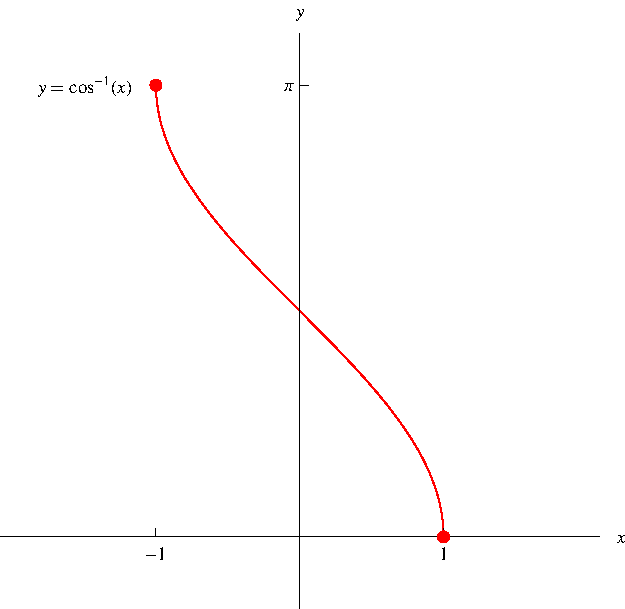
\includegraphics[height=6cm]{inverse-trig/pictures/07-06-arccosd.pdf}%
\column{.5\textwidth}
\begin{enumerate}
\item  \alert<handout:0| 2-3>{Domain: \uncover<3->{$[-1, 1]$.}}
\item  \alert<handout:0| 4-5>{Range: \uncover<5->{$[0, \pi ]$.}}
\item  $\Arccos x = y \Leftrightarrow \cos y = x$ and $0 \leq y \leq \pi$.
\item  $\Arccos (\cos x) = x$ for $0 \leq x \leq \pi$.
\item  $\cos (\Arccos x) = x$ for $-1 \leq x \leq 1$.
\item  $\frac{\diff}{\diff x} (\cos^{-1} x) = -\frac{1}{\sqrt{1-x^2}}$.  \uncover<6->{(The proof is similar to the proof of the formula for the derivative of $\sin^{-1} x$.)}
\end{enumerate}
\end{columns}
\end{frame}
% end module arccos-properties

% begin module arctan-def
\begin{frame}
\begin{columns}[c]
\column{.5\textwidth}
\psset{xunit=0.6cm, yunit=0.6cm}
\begin{pspicture}(-3.9, -3.8)(5.2,3.8)
\psframe*[linecolor=white](-3.9,3.8)(5.2,3.8)
\tiny
\fcAxesStandard{-3.85}{-3.7}{5.2}{3.7}
%Function formula: \frac{\sin{}x}{\cos{}x}
\uncover<handout:0|1>{\psplot[linecolor=\fcColorGraph, plotpoints=1000]{-3.8}{-1.841592654}{x 57.29578 mul tan }}
\uncover<handout:0|1-2>{\psplot[linecolor=\fcColorGraph, plotpoints=1000]{-1.3}{1.3}{x 57.29578 mul tan }}
\uncover<3->{\psplot[linecolor=gray, plotpoints=1000]{-1.3}{1.3}{x 57.29578 mul tan }}
\uncover<handout:0|1>{\psplot[linecolor=\fcColorGraph, plotpoints=1000]{1.841592654}{4.441592654}{x 57.29578 mul tan }}
\uncover<handout:1|3>{\psline[linecolor=blue, linestyle=dashed](-3.65, -3.65)(3.65, 3.65)}
\uncover<handout:0|3>{\psplot[linecolor=\fcColorGraph, plotpoints=1000]{-3.602102448}{3.602102448}{x ATAN }}
\uncover<4->{\psplot[linecolor=\fcColorGraph, plotpoints=1000]{-3.8}{5.15}{x ATAN }}
\uncover<handout:0|1-2>{
\psline[linestyle=dashed](1.570796327, -3.7)(1.570796327, 3.7)
\psline[linestyle=dashed](-1.570796327, -3.7)(-1.570796327, 3.7)
}
\uncover<handout:1|3->{
%\psline[linecolor=gray!20, linestyle=dashed](1.570796327, -3.7)(1.570796327, 3.7)
%\psline[linecolor=gray!20, linestyle=dashed](-1.570796327, -3.7)(-1.570796327, 3.7)
\psline[linestyle=dashed](-3.7, 1.570796327)(5, 1.570796327)
\psline[linestyle=dashed](-3.7, -1.570796327)(5, -1.570796327)
}
\uncover<handout:0|1>{\psline[linestyle=dashed](4.71238898, -3.7)(4.71238898, 3.7)}
\uncover<3->{
\psline(1.570796327, -0.1)(1.570796327, 0.1)
\psline(-1.570796327, -0.1)(-1.570796327, 0.1)
}
\rput[tr](1.5,-0.1){$\frac{\pi}{2}$}
\rput[tr](-1.7,-0.1){$-\frac{\pi}{2}$}
\uncover<handout:0|1>{
\fcXTickWithLabel{3.141592654}{$\pi$}
\fcXTickWithLabel{-3.141592654}{$-\pi$}
}
\uncover<handout:0|1>{\rput[tr](4.65,-0.1){$\frac{3\pi}{2}$}}
\fcYTickWithLabel{1}{$1$}
\fcYTickWithLabel{-1}{$-1$}
\rput[l](1.6, 2.1){ $\begin{array}{l} y=\tan x\uncover<2->{,}\\ \uncover<2->{-\frac{\pi}{2}\leq x\leq\frac{\pi}{2} }\end{array}$
}
\end{pspicture}

%\ \only<handout:0| -1>{%
%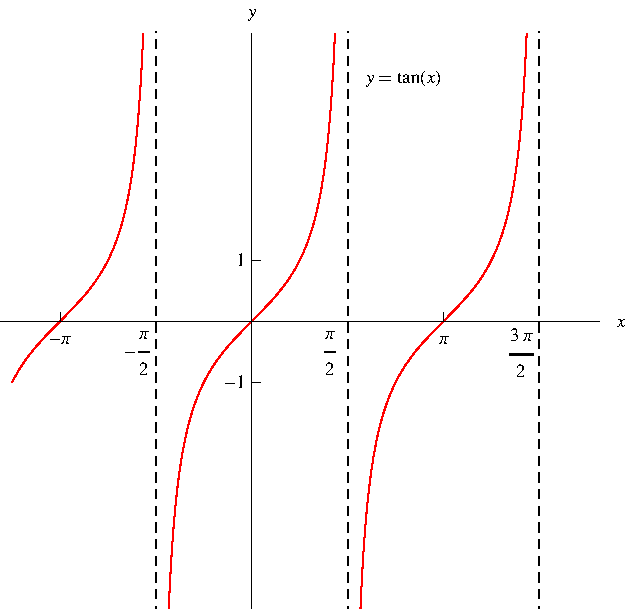
\includegraphics[width=5cm]{inverse-trig/pictures/07-06-arctana.pdf}%
%}%
%\only<handout:1| 2>{%
%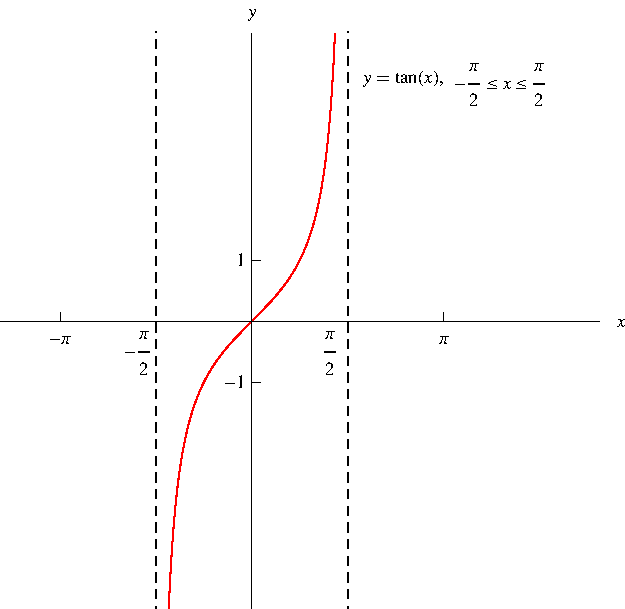
\includegraphics[width=5cm]{inverse-trig/pictures/07-06-arctanb.pdf}%
%}%
%\only<handout:2| 3->{%
%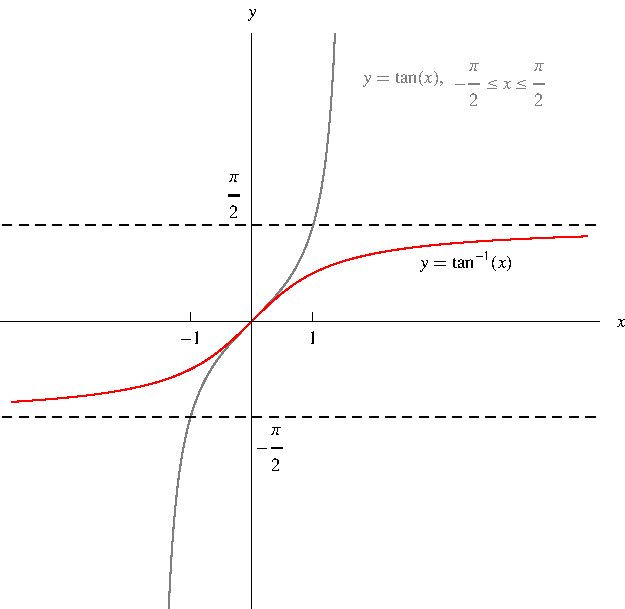
\includegraphics[width=5cm]{inverse-trig/pictures/07-06-arctanc.pdf}%
%}%
\column{.5\textwidth}
\begin{itemize}
\item<1->  $\tan x$ isn't one-to-one.
\item<2->  Restrict the domain to $(-\frac{\pi}2, \frac{\pi}2)$.
\item<3->  The inverse is called $\tan^{-1}$ or $\arctan$.
\item<4->  $\Arctan x = y \Leftrightarrow \tan y = x$ and $-\frac{\pi}2 < y < \frac{\pi}2$.
\item<5->  \alert<handout:0| 5-6>{Domain of $\Arctan$: \uncover<6-| handout:0>{$(-\infty,\infty)$.}}
\item<5->  \alert<handout:0| 7-8>{Range of $\Arctan$: \uncover<8-| handout:0>{$(-\frac{\pi}2, \frac{\pi}2 )$.}}
\item<9->  \alert<handout:0| 9-10>{$\displaystyle \lim_{x\rightarrow \infty} \Arctan x = \uncover<10-| handout:0>{\frac{\pi}2.}$}
\item<9->  \alert<handout:0| 11-12>{$\displaystyle \lim_{x\rightarrow - \infty} \Arctan x = \uncover<12-| handout:0>{- \frac{\pi}2.}$}
\end{itemize}
\end{columns}
\end{frame}
% end module arctan-def



\end{document}
